\documentclass{standalone} 
\usepackage{tzplot}
\usepackage{tikz}
\begin{document}
    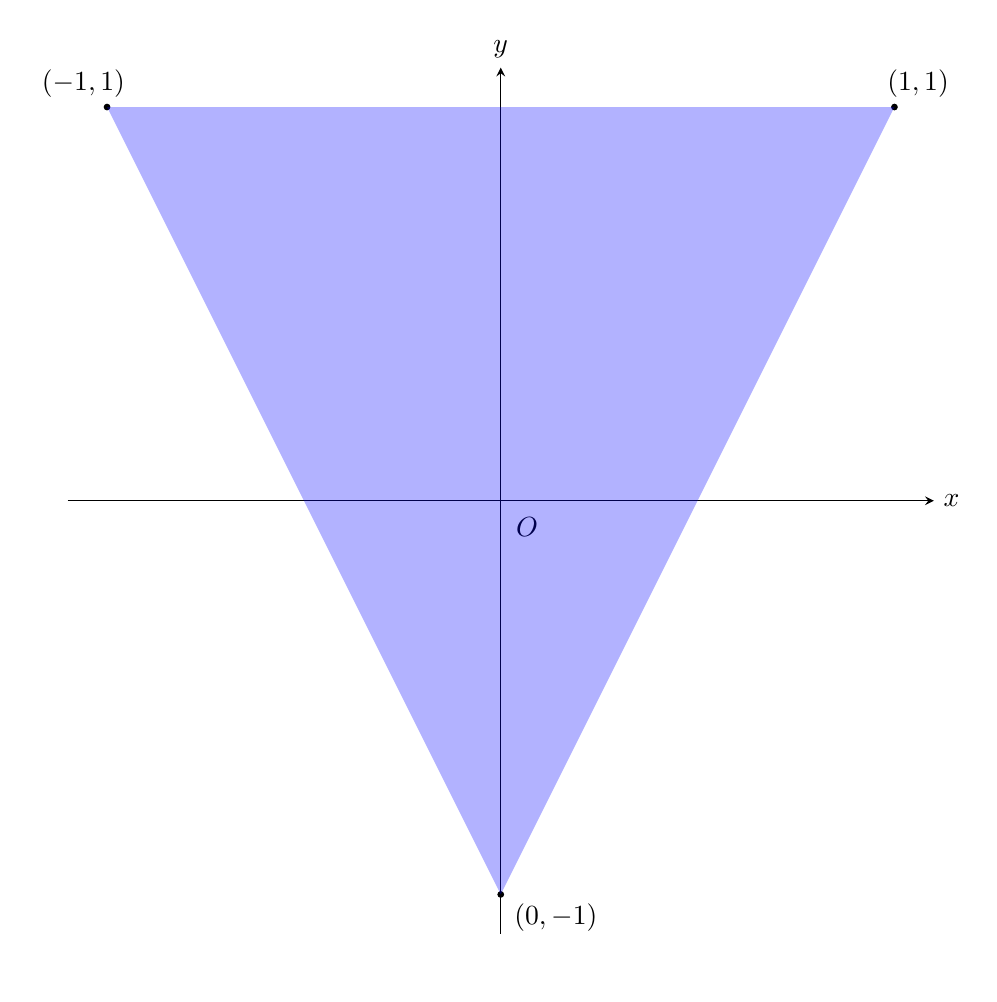
\begin{tikzpicture}
        \tzaxes(-5.5,-5.5)(5.5,5.5){$x$}{$y$}
        
        \node[circle] (o) at (1/3,-1/3){$O$};
        
        \node[circle] (o) at (5.3,5.3){$(1,1)$};
        \fill[draw] (5,5) circle (1pt) coordinate (mark-1);
        \node[circle] (o) at (0.7,-5.3){$(0,-1)$};
        \fill[draw] (0,-5) circle (1pt) coordinate (mark-2);
        \node[circle] (o) at (-5.3,5.3){$(-1,1)$};
        \fill[draw] (-5,5) circle (1pt) coordinate (mark-4);

        \fill[opacity=0.3,blue] (mark-4) --  (mark-1) -- (mark-2) -- cycle;
    \end{tikzpicture}
\end{document}